\documentclass{article}
\usepackage{amsmath}
\usepackage{fullpage}
\usepackage{graphicx}

\title{Spherical Coordinates}
\author{M. en C. Reinaldo Zapata}
\date{}

\begin{document}
\maketitle

\section*{Spherical coordinates} % (fold)
\label{sec:spherical_coordinates}

The use of symbols and the order of the coordinates differs between sources. In
one system frequently encountered in physics ($r$, $\theta$, $\varphi$) gives
the radial distance, polar angle, and azimuthal angle, whereas in another system
used in many mathematics books ($r$, $\theta$, $\varphi$) gives the radial
distance, azimuthal angle, and polar angle.

The coordinates are defines as:
\begin{align*}
r &= \sqrt{x^{2} + y^{2} + z^{2}} & & r \geq 0\\
\theta &= \arccos \left( \frac{z}{r} \right) = 2 \arctan \left( \frac{\sqrt{1- 
(z/r)^{2} }}{1 + z/r} \right) & 0 \leq &\theta \leq \pi \\
\varphi &= \arctan \left( \frac{y}{x} \right) & 0 \leq &\varphi \leq 2\pi \\ \\ 
x &= r \, \sin \theta \, \cos \varphi \\
y &= r \, \sin \theta \, \sin \varphi \\
z &= r \, \cos \theta
\end{align*}


\begin{figure}[h]
    \centering
    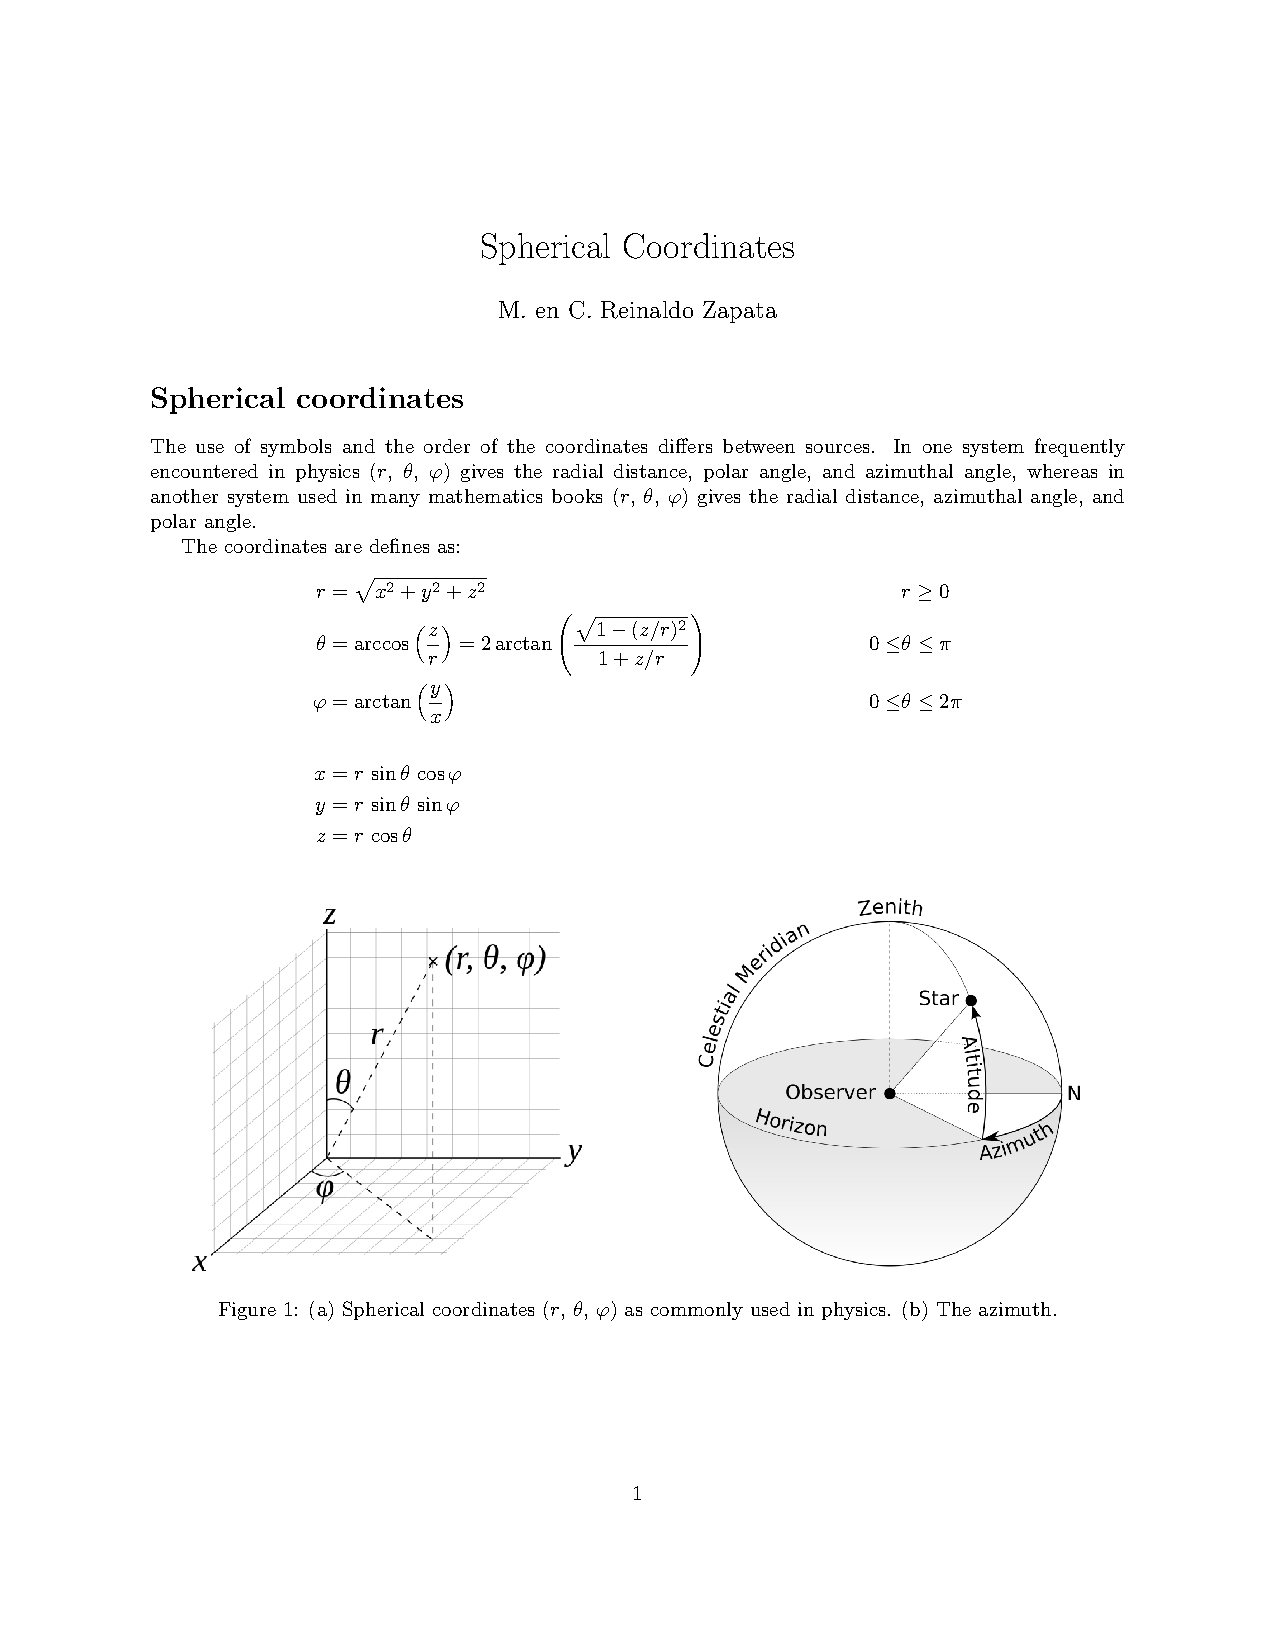
\includegraphics[width=0.4\textwidth]{spherical_coordinates}
    \hspace{0.1\textwidth}
    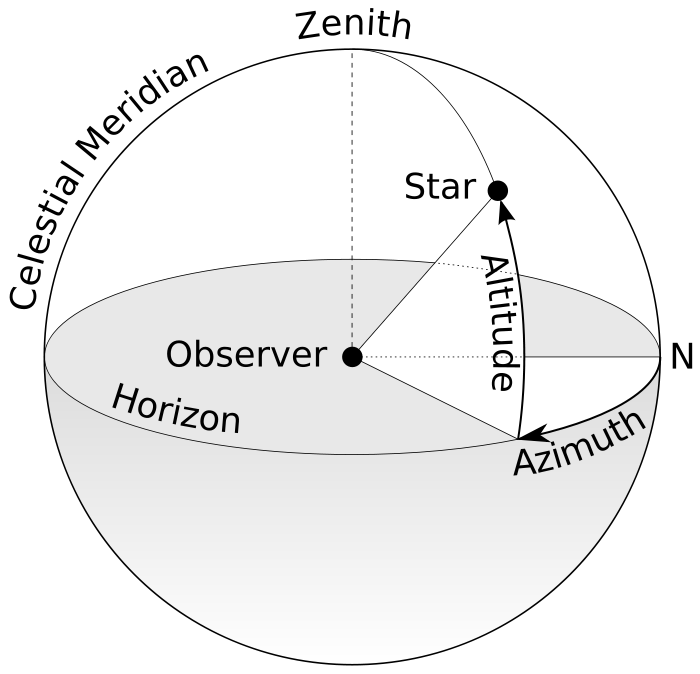
\includegraphics[width=0.4\textwidth]{azimuth}
    \caption{(a) Spherical coordinates ($r$, $\theta$, $\varphi$) as commonly used
    in physics. (b) The azimuth.}
    \label{fig:spherical coordinates}
\end{figure}

% \tt{acos =  atan2(sqrt(1-x*x), x) }


% section spherical_coordinates (end)


\end{document}
